% % % % % % % % % % % % % % % % % % % % % % % % % % % % % % % % % % % % % % % % % % % %
%                                                                                     %
% Short Sectioned Assignment LaTeX Template Version 1.0 (5/5/12)                      %
% This template has been downloaded from: http://www.LaTeXTemplates.com               %
%                                                                                     %
% Original author:  Frits Wenneker (http://www.howtotex.com)                          %
%                                                                                     %
% Modified by: Fco Javier Sueza Rodríguez (fcosueza@disroot.org)                      %
%                                                                                     %
% Changes:                                                                            %
%	    - Custom Chapters, Sections and Subsections (titlesec package)                %
%           - Document type scrbook (oneside)                                         %
%           - Use babel-lang-spanish package and marvosym                             %
%           - Use hyperref, enumitem, tcolorbox and glossaries packages               %
%           - Use Time New Roman (mathptmx), Helvetic and Courier fonts               %
%                                                                                     %
% License: CC BY-NC-SA 3.0 (http://creativecommons.org/licenses/by-nc-sa/3.0/)        %
%                                                                                     %
% % % % % % % % % % % % % % % % % % % % % % % % % % % % % % % % % % % % % % % % % % % %

%-----------------------------------------------%
%	              Packages                  %
%-----------------------------------------------%

\documentclass[paper=a4, fontsize=11pt, oneside]{scrbook}

% ---- Text Input/Output ----- %

\usepackage[T1]{fontenc}
\usepackage[utf8]{inputenc}
\usepackage{mathptmx}
\usepackage[scaled=.92]{helvet}
\usepackage{courier}
\usepackage[indent=12pt]{parskip}

\usepackage{geometry}
\geometry{verbose,tmargin=3cm,bmargin=3cm,lmargin=2.6cm,rmargin=2.6cm}

% ---- Language ----- %

\usepackage[spanish]{babel}
\usepackage{marvosym}

% ---- Another packages ---- %

\usepackage{amsmath,amsfonts,amsthm}
\usepackage{graphics,graphicx}
\usepackage{titlesec}
\usepackage{fancyhdr}
\usepackage{tcolorbox}
\usepackage{hyperref}
\usepackage{enumitem}
\usepackage[automake]{glossaries}

%--------------------------------------------------------------------%
%                      Customizing Document                          %
%--------------------------------------------------------------------%


% ----------- Custom Chapters, Sections and Subsections -------------- %

\titleformat{\chapter}[display]
			{\bfseries\Huge}
			{Tema \ \thechapter} {0.5ex}
			{\vspace{1ex}\centering}

\titleformat{\section}[hang]
			{\bfseries\Large}
			{\thesection}{0.5em}{}

\titleformat{\subsection}[hang]
			{\bfseries\large}
			{\thesubsection}{0.5em}{}

\titleformat{\subsubsection}[hang]
			{\bfseries\large}
			{\thesubsubsection}{0.5em}{}

\hypersetup{
    colorlinks=true,
    linkcolor=black,
    urlcolor=magenta
}

% ------------------- Custom heaaders and footers ------------------- %

\pagestyle{fancyplain}

\fancyhead[]{}
\fancyfoot[L]{}
\fancyfoot[C]{}
\fancyfoot[R]{\thepage}

\renewcommand{\headrulewidth}{0pt} % Remove header underlines
\renewcommand{\footrulewidth}{0pt} % Remove footer underlines

\setlength{\headheight}{13.6pt} % Customize the height of the header

% --------- Numbering equations, figures and tables ----------------- %

\numberwithin{equation}{section} % Number equations within sections
\numberwithin{figure}{section} % Number figures within sections
\numberwithin{table}{section} % Number tables within sections

% ------------------------ New Commands ----------------------------- %

\newcommand{\horrule}[1]{\rule{\linewidth}{#1}} % Create horizontal rule command


%----------------------------------------------------------------------------------------
%	TÍTULO Y DATOS DEL ALUMNO
%----------------------------------------------------------------------------------------

\title{
\vspace{10ex}
\normalfont \normalsize
\Huge \textbf{Tarea 7: Uso de Bases de Datos Objeto-Relacionales}
}
\author{Francisco Javier Sueza Rodríguez}
\date{\normalsize\today}

%----------------------------------------------------------------------------------------
%                                     DOCUMENTO
%----------------------------------------------------------------------------------------
\begin{document}

\maketitle

\thispagestyle{empty}

\vspace{62ex}

\begin{center}
    \begin{tabular}{l l}
        \textbf{Centro}: & IES Aguadulce \\
        \textbf{Ciclo Formativo}: & Desarrollo Aplicaciones Web (Distancia)\\
        \textbf{Asignatura}: & Bases de Datos\\
        \textbf{Tema}: & Tema 7 - Uso de Bases de Datos Objeto-Relacionales\\
    \end{tabular}
\end{center}

\newpage

\tableofcontents

\newpage

\listoffigures

\newpage

\section{Caso Práctico}
Una organización sin ánimo de lucro llamada LA CESTA SOLIDARIA ofrece la posibilidad de repartir alimentos a las personas que más lo necesiten. Para ello, los alimentos que los ceden gratuitamente empresas y particulares se organizan en cestas con diferentes tipos de productos y los voluntarios se encargan de repartirlas a los clientes o socios que acuden al almacén registrándose para ello con los datos personales, renta y miembros en la unidad familiar.

Hasta ahora, todo lo que hemos visto ha sido sobre bases de datos relacionales, sin embargo la aparición de las bases de datos orientadas a objetos nos ofrece nuevas perspectivas para aprovechar de manera más óptima las bases de datos.

De esta manera se trata  es de ver las ventajas que nos ofrecen este tipo de bases de datos principalmente en aspectos como  la reutilización de código, el trabajo colaborativo, y la interconexión de las bases de datos con otros lenguajes de programación orientados a objetos.

Como Juan ha realizado recientemente un curso de bases de datos orientadas a objetos, Ada le ha propuesto a él que utilizando los conocimientos adquiridos en el curso realice la base de datos orientada a objetos que tienen que desarrollar para la gestión de esta organización.

\section{Actividades}
El propósito de esta tarea es crear los objetos, tablas y bloques de código necesarios para crear la BD objeto-relacional que se propone a continuación y probarla mediante la creación de instancias creadas a partir de esos objetos.


En la organización \textbf{LA CESTA SOLIDARIA }se  desea informatizar la gestión de los voluntarios que reparten diferentes donaciones en forma de cestas con productos a los clientes o socios más vulnerables dependiendo del tipo de ayuda que necesiten. Tú también puedes colaborar con esta organización informatizando una BD objeto-relacional que maneje la funcionalidad que nos solicitan. Para ello debes crear los objetos y tablas siguientes.

\subsection{Actividad 1}

\subsubsection{Enunciado}
Realiza los siguientes subapartados:

\begin{enumerate}[label=\alph*)]
    \item Crea el tipo de objeto ``\textbf{Persona}'' con los siguientes atributos teniendo en cuenta que otros objetos heredarán de éste:

 \begin{figure}[H]
     \begin{tcolorbox}[sharp corners, colback=yellow!30, colframe=white!20]
         \scriptsize
         \begin{verbatim}
     DNI       VARCHAR2(9),
     nombre    VARCHAR2(30),
     apellidos VARCHAR2(40),
     telefono  VARCHAR2(9),
     f_ingreso DATE\end{verbatim}
     \end{tcolorbox}
 \end{figure}

 \item  Crea, como tipo heredado de ``\textbf{Persona}'', el tipo de objeto ``\textbf{Voluntario}'' con los siguientes atributos:

  \begin{figure}[H]
     \begin{tcolorbox}[sharp corners, colback=yellow!30, colframe=white!20]
         \scriptsize
         \begin{verbatim}
     puntosAcumula NUMBER(8)\end{verbatim}
     \end{tcolorbox}
 \end{figure}

    Y el siguiente método:

    \begin{itemize}
        \item \textbf{calcularPuntosGanados}: que devolverá la cantidad resultante de multiplicar los turnos del mes que ha colaborado en la organización por 50.
    \end{itemize}

    \item Crea, como tipo heredado de ``\textbf{Persona}'', el tipo de objeto ``\textbf{Cliente}'' con los siguientes atributos:

 \begin{figure}[H]
    \begin{tcolorbox}[sharp corners, colback=yellow!30, colframe=white!20]
        \scriptsize
        \begin{verbatim}
        ingresosMes NUMBER(6,2),
        miembrosFam NUMBER(2),
        tipoAyuda   VARCHAR2(1)\end{verbatim}
    \end{tcolorbox}
\end{figure}

     Y el siguiente método constructor:
     \begin{itemize}
         \item \textbf{Cliente(parámetos\_necesarios)} : el valor del atributo tipoAyuda se inicializará de forma automática cuando se cree una instancia mediante este constructor en el que se pasan como parámetros necesarios todos los atributos excepto el de tipoAyuda que deberá inicializarse automáticamente de la siguiente forma:
         \begin{itemize}
             \item Si la renta es menor o igual que 50 el atributo tipoAyuda es A
             \item Si la renta es mayor que 50 y menor o igual que 100 el atributo tipoAyuda es B.
             \item Si la renta es mayor que 100 entonces el atributo tipoAyuda es C.

             Para calcular la renta se necesitarán los datos ingreso mensual y miembros de la unidad familiar del cliente. La fórmula sería la siguiente:

               \begin{figure}[H]
                 \begin{tcolorbox}[sharp corners, colback=yellow!30, colframe=white!20]
                     \scriptsize
                     \begin{verbatim}
                         renta = ingresosMes/miembrosFam\end{verbatim}
                 \end{tcolorbox}
             \end{figure}
         \end{itemize}
     \end{itemize}
\end{enumerate}

\subsubsection{Solución}
En este apartado vamos a empezar a crear los \textbf{tipos de objetos} que vamos a usar en nuestra base de datos:

\begin{enumerate}[label=\alph*)]
    \item En primer lugar hemos creado el objeto \textbf{Persona}, como podemos ver en la siguiente imagen.

    \begin{figure}[H]
        \centering
        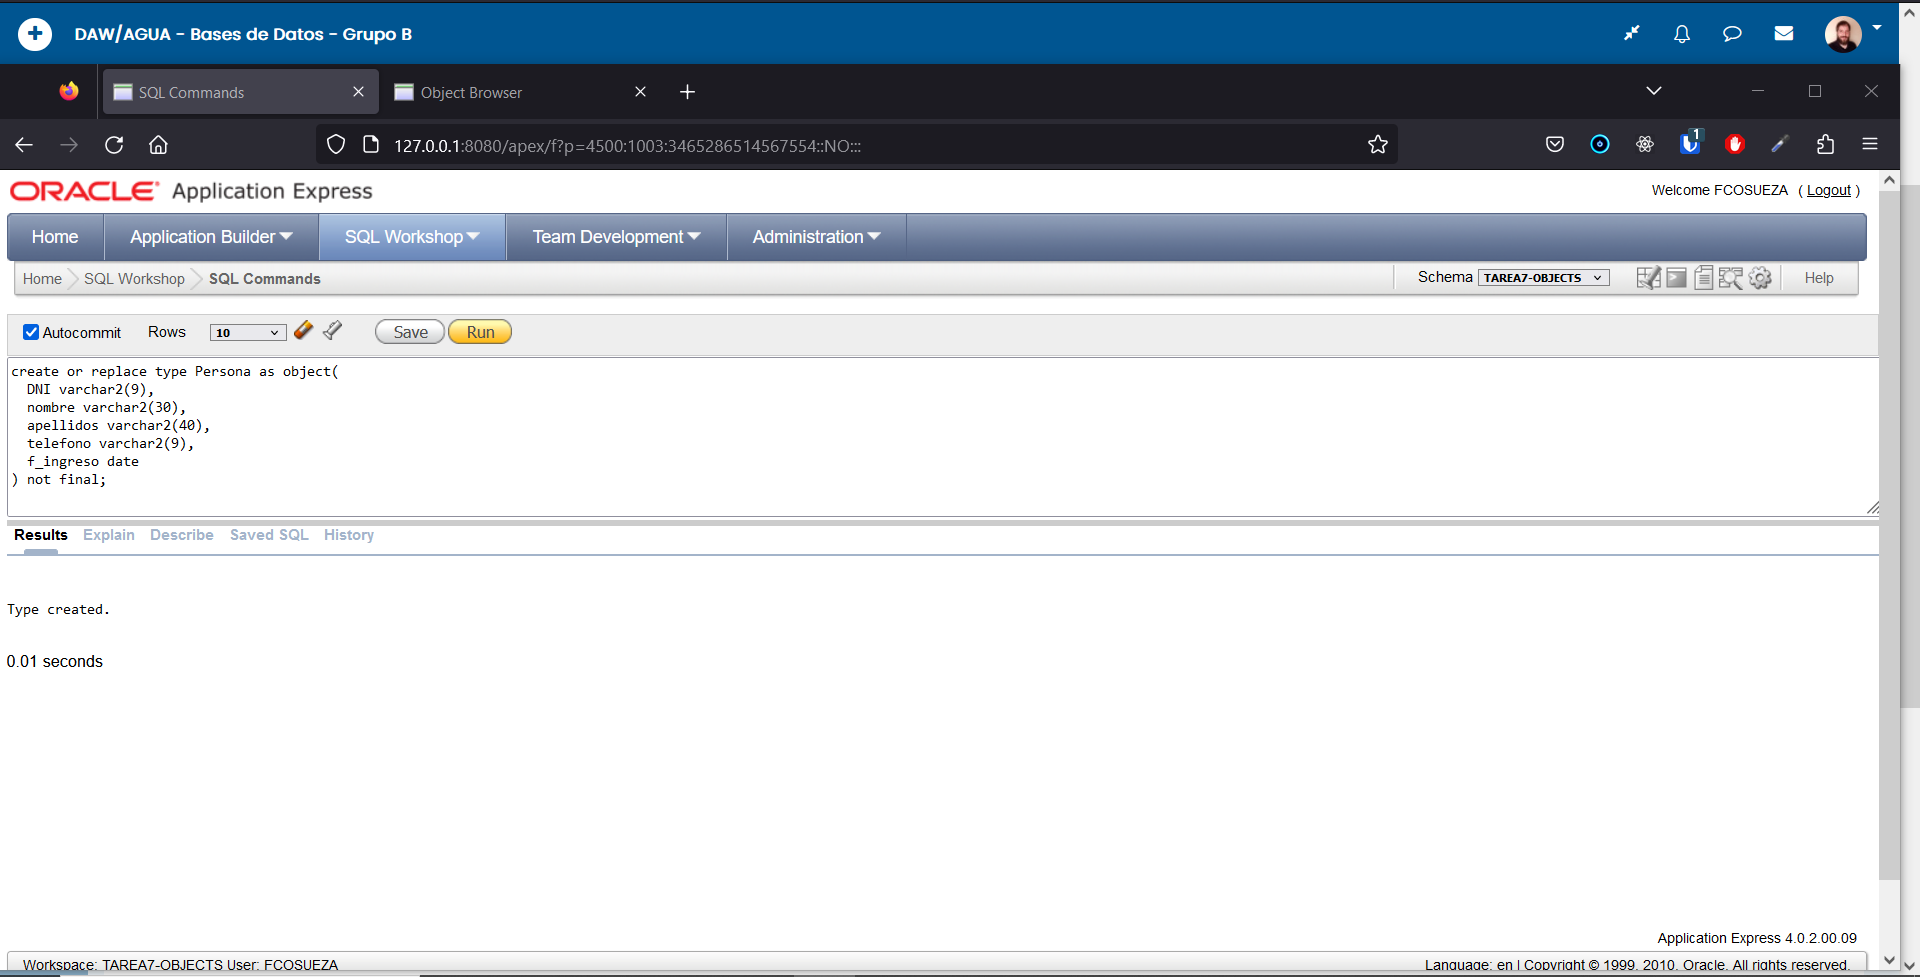
\includegraphics[scale=0.30]{creacion-persona.png}
        \caption{Creación del Objeto Persona}
    \end{figure}

    Hemos creado este objeto con los datos proporcionados, añadiendo \textbf{NOT FINAl} al final, para indicar que va a ser un objeto del que van ha heredar otros. El código empleado para su definición ha sido el siguiente:

    \begin{figure}[H]
        \begin{tcolorbox}[sharp corners, colback=yellow!30, colframe=white!20]
            \tiny
            \begin{verbatim}
CREATE OR REPLACE TYPE PERSONA as object(
  DNI varchar2(9),
  nombre varchar2(30),
  apellidos varchar2(40),
  telefono varchar2(9),
  f_ingreso date
) not final
            \end{verbatim}
        \end{tcolorbox}
    \end{figure}

    \item El siguiente objeto creado ha sido el tipo \textbf{Voluntario}, el cual es un tipo \textbf{hijo} de Persona, lo que hemos indicado con la palabra \textbf{UNDER} en su definición, como podemos ver en la siguiente captura.

    \begin{figure}[H]
        \centering
        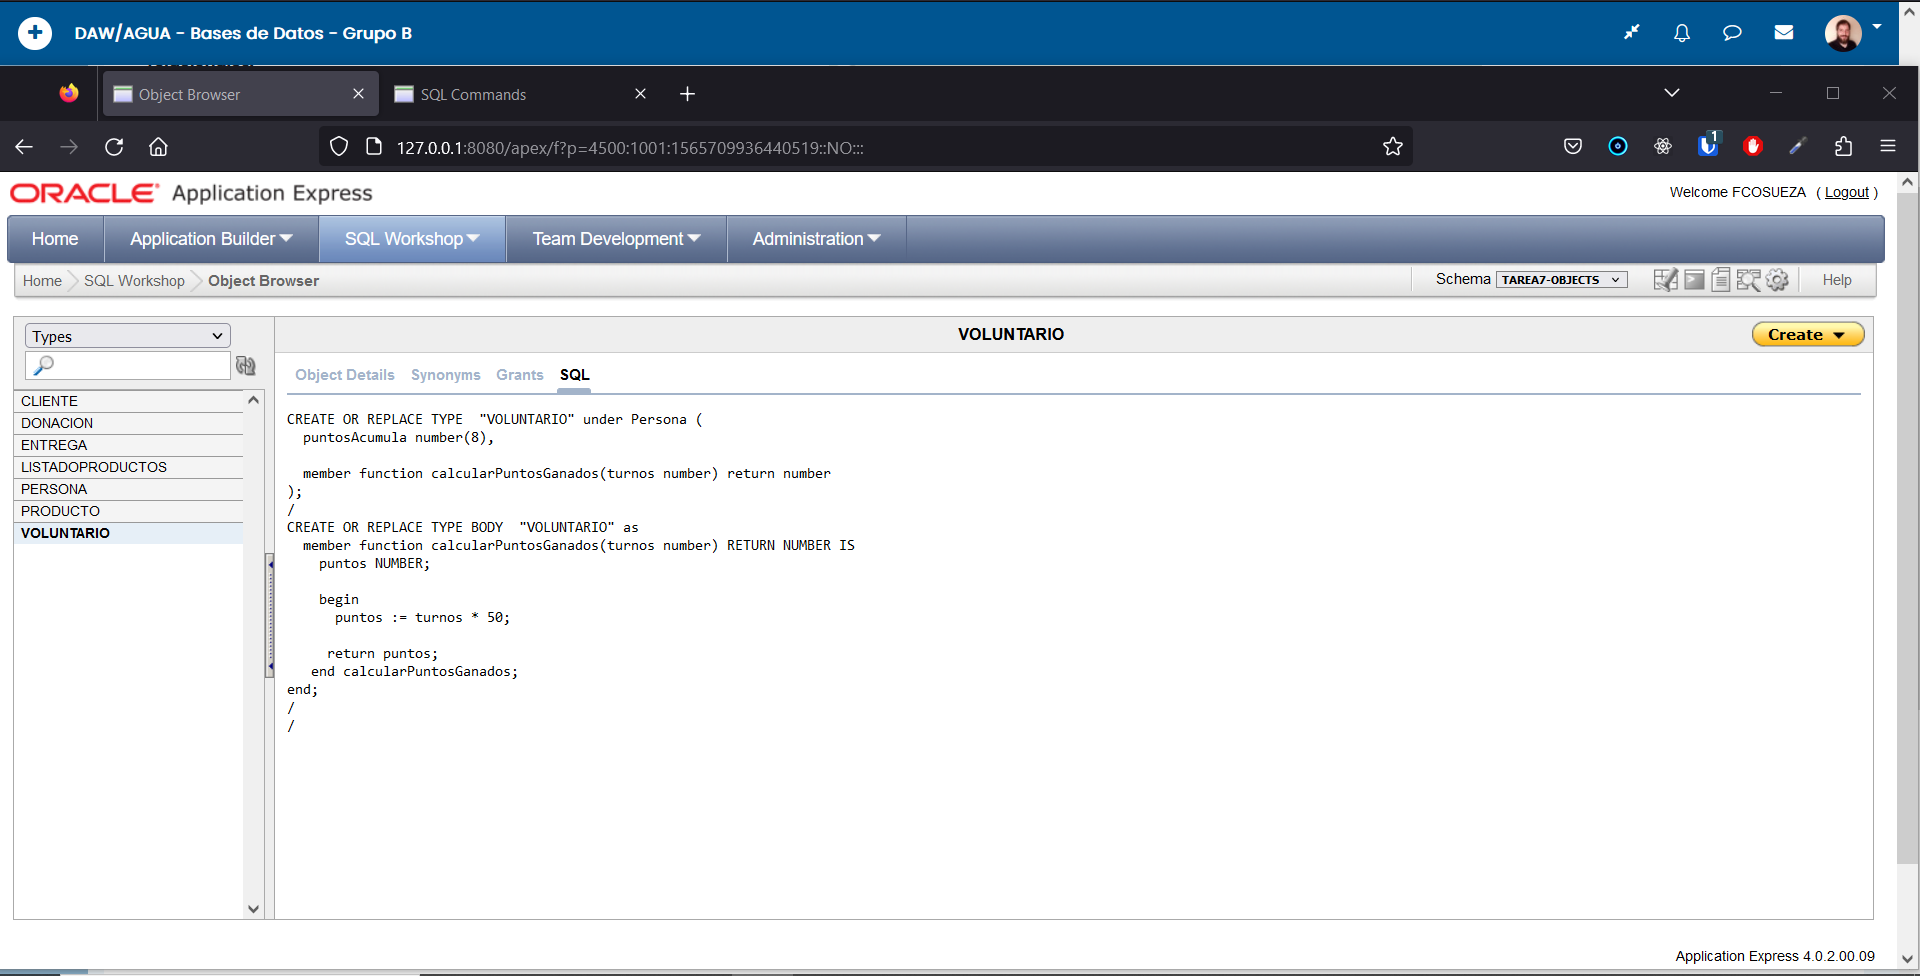
\includegraphics[scale=0.30]{creacion-voluntario.png}
        \caption{Creación del Objeto Voluntario}
    \end{figure}

    Además, este objeto incorpora un \textbf{método} para calcular los puntos que ha ganado un voluntario según la cantidad de turnos que ha realizado en el mes, lo cual hemos definido dentro de su correspondiente \textbf{TYPE BODY}. El código empleado ha sido el siguiente.

    \begin{figure}[H]
        \begin{tcolorbox}[sharp corners, colback=yellow!30, colframe=white!20]
            \tiny
            \begin{verbatim}

CREATE OR REPLACE TYPE  VOLUNTARIO under Persona (
  puntosAcumula number(8),

  member function calcularPuntosGanados(turnos number) return number
);
/

CREATE OR REPLACE TYPE BODY VOLUNTARIO as
  member function calcularPuntosGanados(turnos number) RETURN NUMBER IS

  puntos NUMBER;

  begin
    puntos := turnos * 50;

    return puntos;
  end calcularPuntosGanados;
end;\end{verbatim}
        \end{tcolorbox}
    \end{figure}

    \item EL siguiente objeto creado ha sido el objeto \textbf{Cliente}, que además de hededar de persona, tiene un constructor propio, como podemos ver en el código empleado a continuación.

    \begin{figure}[H]
        \begin{tcolorbox}[sharp corners, colback=yellow!30, colframe=white!20]
            \tiny
            \begin{verbatim}
CREATE OR REPLACE TYPE CLIENTE UNDER Persona(
ingresosMes NUMBER(6,2),
miembrosFam NUMBER(2),
tipoAyuda VARCHAR2(1),

CONSTRUCTOR FUNCTION Cliente(
DNI VARCHAR2,
nombre VARCHAR2,
apellidos VARCHAR2,
telefono VARCHAR2,
f_ingreso DATE,
ingresosMes NUMBER,
miembrosFam NUMBER
) RETURN self AS result
);
/

-- Definición del constructor Cliente que calcula automáticamente el valor de tipoAyuda

CREATE OR REPLACE TYPE BODY CLIENTE AS
CONSTRUCTOR FUNCTION Cliente(
DNI VARCHAR2,
nombre VARCHAR2,
apellidos VARCHAR2,
telefono VARCHAR2,
f_ingreso DATE,
ingresosMes NUMBER,
miembrosFam NUMBER
) RETURN self AS result IS

renta NUMBER;

BEGIN
SELF.DNI := DNI;
SELF.nombre := nombre ;
SELF.apellidos := apellidos;
SELF.telefono := telefono;
SELF.f_ingreso := f_ingreso;
SELF.ingresosMes := ingresosMes;
SELF.miembrosFam := miembrosFam;

renta := ingresosMes / miembrosFam;

IF (renta <= 50) THEN
SELF.tipoAyuda := 'A';
ELSIF (renta <= 100) THEN
SELF.tipoAyuda := 'B';
ELSE
SELF.tipoAyuda := 'C';
END IF;

RETURN;
END;

END;
            \end{verbatim}
        \end{tcolorbox}
    \end{figure}
\end{enumerate}

\subsection{Actividad 2}

\subsubsection{Enunciado}
Realiza los siguientes subapartados:

\begin{enumerate}[label=\alph*)]
    \item Crea el tipo de objeto ``\textbf{Producto}'' con los siguientes atributos:

     \begin{figure}[H]
        \begin{tcolorbox}[sharp corners, colback=yellow!30, colframe=white!20]
            \scriptsize
            \begin{verbatim}
          codigo   VARCHAR2(3),
          nombre   VARCHAR2(30),
          cantidad NUMBER(3)
          medida   VARCHAR2(10)\end{verbatim}
        \end{tcolorbox}
    \end{figure}

    \item Crea una colección VARRAY llamada \textbf{ListadoProductos} en la que se puedan almacenar hasta 20 objetos de tipo Productos.

    \item Crea el tipo de objeto ``\textbf{Donacion}'' con los siguientes atributos:

     \begin{figure}[H]
    \begin{tcolorbox}[sharp corners, colback=yellow!30, colframe=white!20]
        \scriptsize
        \begin{verbatim}
          numero     VARCHAR2(3),
          valor      NUMBER(6,2),
          listaCesta ListadoProductos\end{verbatim}
    \end{tcolorbox}
\end{figure}

    \item Crea el tipo de objeto ``\textbf{Entrega}'' con los siguientes atributos:

    \begin{figure}[H]
        \begin{tcolorbox}[sharp corners, colback=yellow!30, colframe=white!20]
            \scriptsize
            \begin{verbatim}
         numero     VARCHAR2(5),
         fecha      DATE,
         socio      Cliente,
         repartidor REF Voluntario,
         cesta      Donacion\end{verbatim}
        \end{tcolorbox}
    \end{figure}
\end{enumerate}

\subsubsection{Solución}
Puede ver el código de la solución en el archivo adjunto, no me ha dado tiempo a realizar la explicación. :(

\subsection{Actividad 3}

\subsubsection{Enunciado}
Crea las siguientes tablas de objetos con la sentencia apropiada para cada uno de los subapartados:

\begin{enumerate}[label=\alph*)]
    \item Una tabla llamada VOLUNTARIADO de objetos tipo Voluntario.
    \item Una tabla llamada SOCIOS de objetos tipo Cliente.
    \item Una tabla llamada CATALOGO de objetos tipo Producto.
    \item Una tabla llamada ENTREGADOS de objetos tipo Entrega.
\end{enumerate}

\subsubsection{Solución}
En este aparatado hemos creado las diferentes tablas, usando para ello el siguiente código:

\begin{figure}[H]
    \begin{tcolorbox}[sharp corners, colback=yellow!30, colframe=white!20]
        \tiny
        \begin{verbatim}
CREATE TABLE VOLUNTARIADO OF  VOLUNTARIO;
CREATE TABLE SOCIOS OF CLIENTE;
CREATE TABLE CATALOGO OF PRODUCTO;
CREATE TABLE ENTREGADOS OF ENTREGA;
        \end{verbatim}
    \end{tcolorbox}
\end{figure}

\subsection{Actividad 4}
Para trabajar con los objetos y tablas creados debes usar instancias y bloques de PL/SQL. A continuación debes implementar \textbf{diferentes bloques PL/SQL} con lo que se pide \textbf{en cada uno de los siguientes subapartados}:

\begin{enumerate}[label=\alph*)]
    \item Crea \textbf{dos} instancias de Voluntario con los siguientes datos:

     \begin{figure}[H]
        \centering
        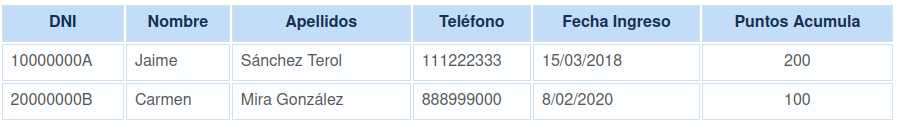
\includegraphics[scale=0.60]{datos-voluntariado.png}
     \end{figure}

    A continuación y dentro del mismo bloque realiza las siguientes acciones:
    \begin{itemize}
        \item Inserta las instancias en la tabla VOLUNTARIADO.
        \item Utiliza el método que has creado en este objeto para calcular los puntos ganados por el voluntario con DNI 10000000A sabiendo que ha colaborado 8 turnos en un mes.
        \item Por último, actualiza en la tabla VOLUNTARIADO el valor correspondiente a este voluntario incrementando los puntos ganados a su acumulado.
    \end{itemize}

    \item Crea \textbf{tres} instancias de Cliente con los siguientes datos y después debes insertarlos en la tabla SOCIOS.

    \begin{figure}[H]
        \centering
        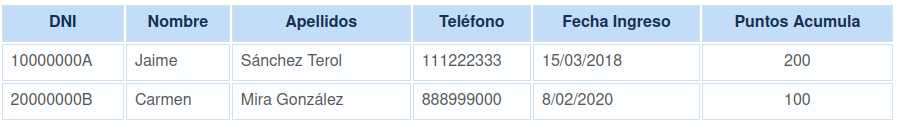
\includegraphics[scale=0.60]{datos-voluntariado.png}
    \end{figure}

    \item Crea \textbf{ocho} instancias de Producto con los siguientes datos e insértalos en la tabla CATALOGO.

    \begin{figure}[H]
        \centering
        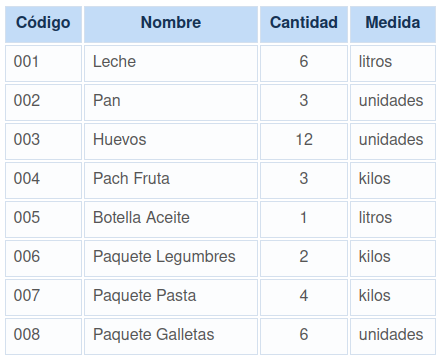
\includegraphics[scale=0.60]{datos-producto.png}
    \end{figure}

    A continuación en ese mismo bloque PL/SQL realiza las siguientes acciones:

    \begin{itemize}
        \item Crea \textbf{tres} instancias de ListadoProductos con los siguientes datos:
        \begin{itemize}
            \item ListaProductos1 contiene los objetos de tipo Producto : 001,003,005 y 007.
            \item ListaProductos2 contiene los objetos de tipo Producto: 001,002,004 y 008.
            \item ListaProductos3 contiene los objetos de tipo Producto: 003,005 y 006.
        \end{itemize}

        \item Muestra en un mensaje por pantalla los nombres de todos los productos que forman la ListaProductos1 accediendo a dicha lista y recuperando esa información. Nota: NO hay que obtenerlos de las instancias propias de Producto sino de la instancia ListaProductos1 que almacena dichos elementos en el orden insertado. Visita el siguiente enlace para ver qué métodos se pueden emplear en las colecciones.

        \item Crea tres instancias de Donacion con los siguientes datos:

    \begin{figure}[H]
    \centering
    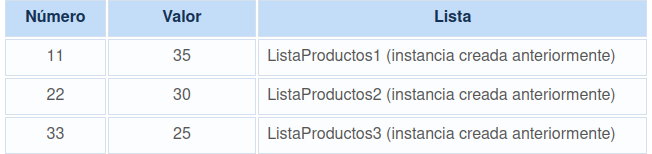
\includegraphics[scale=0.60]{datos-donaciones.png}
    \end{figure}

    \item Obtén la referencia de cada voluntario almacenado en la tabla correspondiente y guarda dichas referencias en variables del tipo apropiado.
    \item Obtén las instancias de los clientes 11111111A y 22222222B almacenados en la tabla correspondiente y guárdalos en variables del tipo apropiado.
    \item A continuación crea \textbf{cuatro} instancias de Entrega con la siguiente información teniendo en cuenta que:
    \begin{itemize}
        \item en el atributo  Socio debes insertar la instancia recuperada de cliente que se indica a continuación.
        \item en el atributo Repartidor debes insertar la referencia del objeto voluntario recuperada correspondiente.
        \item en el atributo Cesta debes insertar el objeto creado como instancias de Donacion que se indica a continuación.

        \begin{figure}[H]
            \centering
            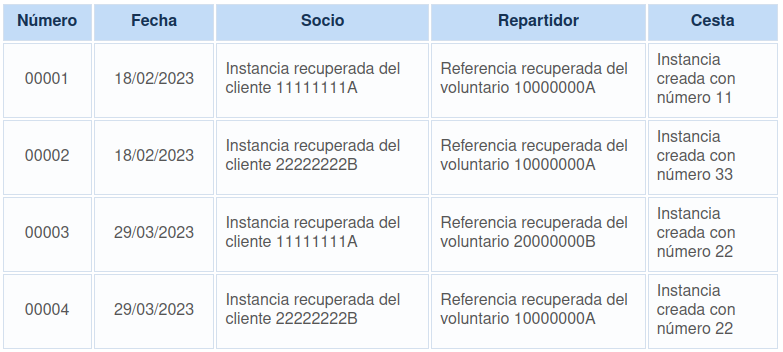
\includegraphics[scale=0.60]{datos-cesta.png}
        \end{figure}
    \end{itemize}

      \item Para finalizar el bloque, una vez creadas las cuatro instancias debes insertarlas en la tabla ENTREGADOS.
    \end{itemize}
\end{enumerate}

\subsubsection{Solución}
En este ejercicio hemos empezado a trabajar ya con las tablas creadas y nuestros tipos de objetos.

\begin{enumerate}[label=\alph*)]
    \item En primer lugar hemos trabajado con la tabla voluntariado, donde hemos creado dos instancias de objetos \textbf{voluntario} y las hemos insertado como se ve a continuación.

    \begin{figure}[H]
        \centering
        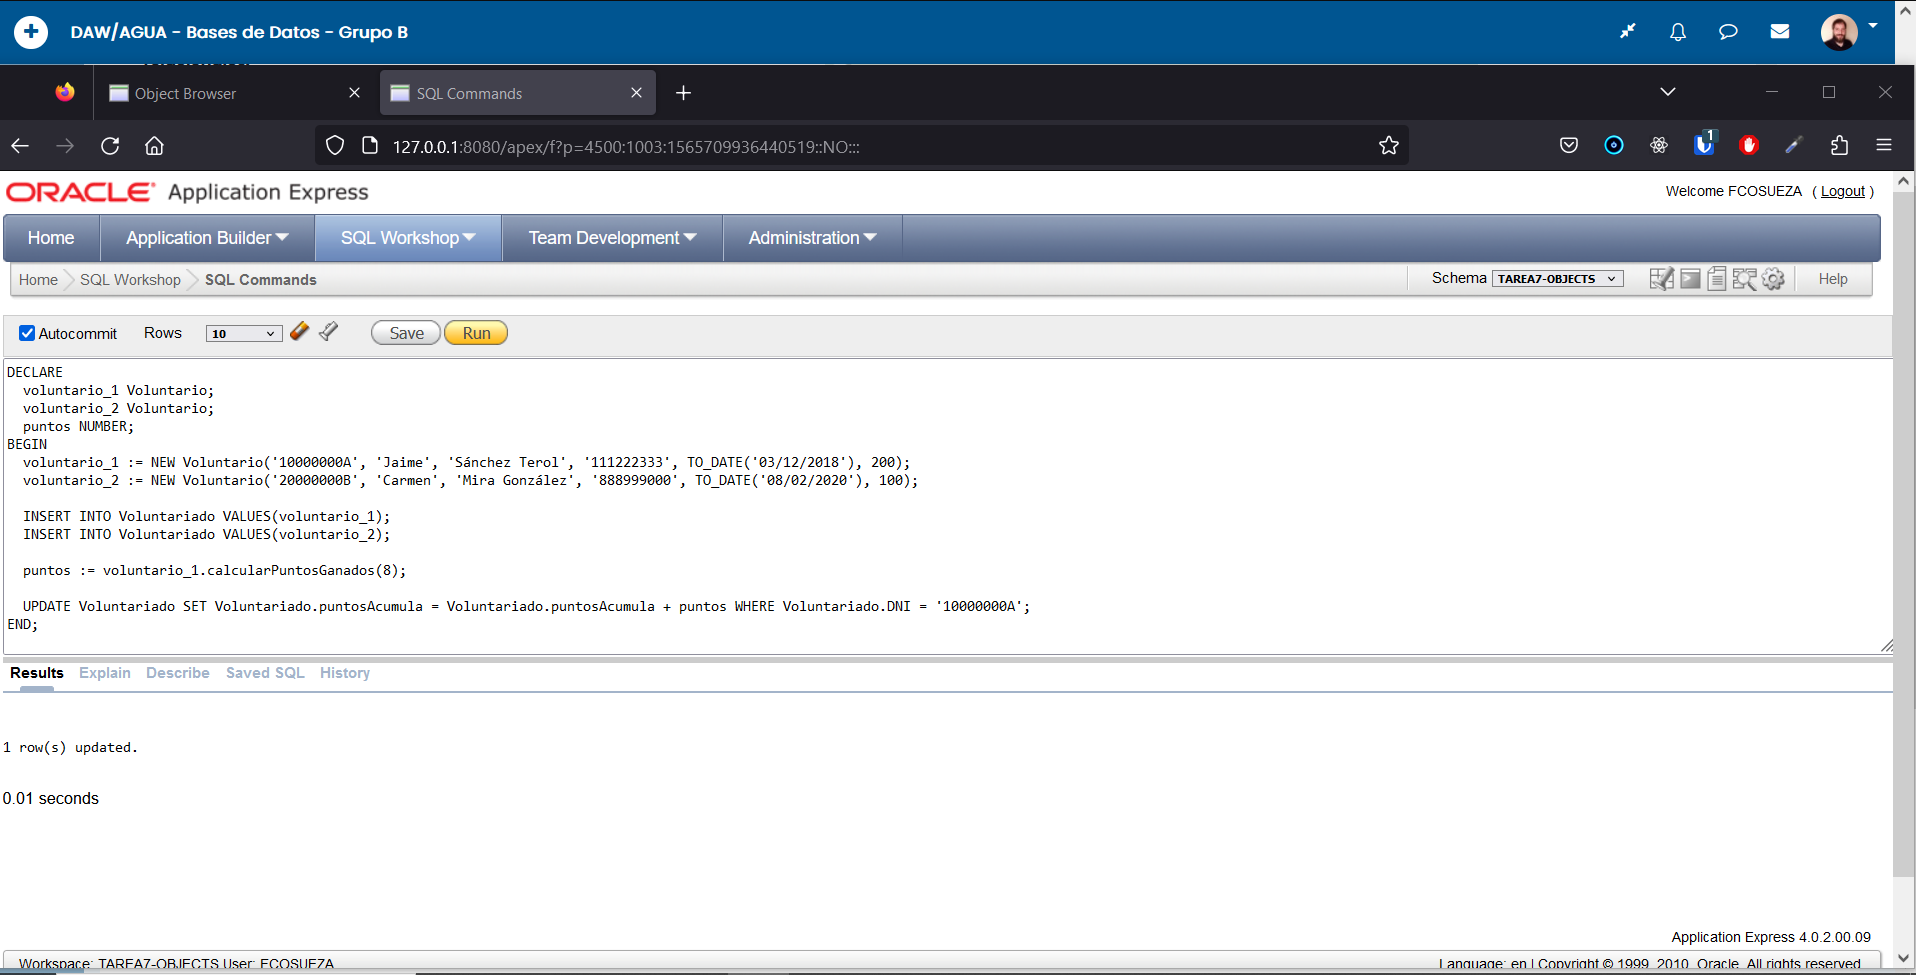
\includegraphics[scale=0.30]{voluntario-op-1.png}
        \caption{Creación e inserción en la tabla Voluntariado}
    \end{figure}

    Hemos realizado un SELECT para comprobar que se habían insertado correctamente los objetos, como podemos ver en la siguiente captura.

    \begin{figure}[H]
        \centering
        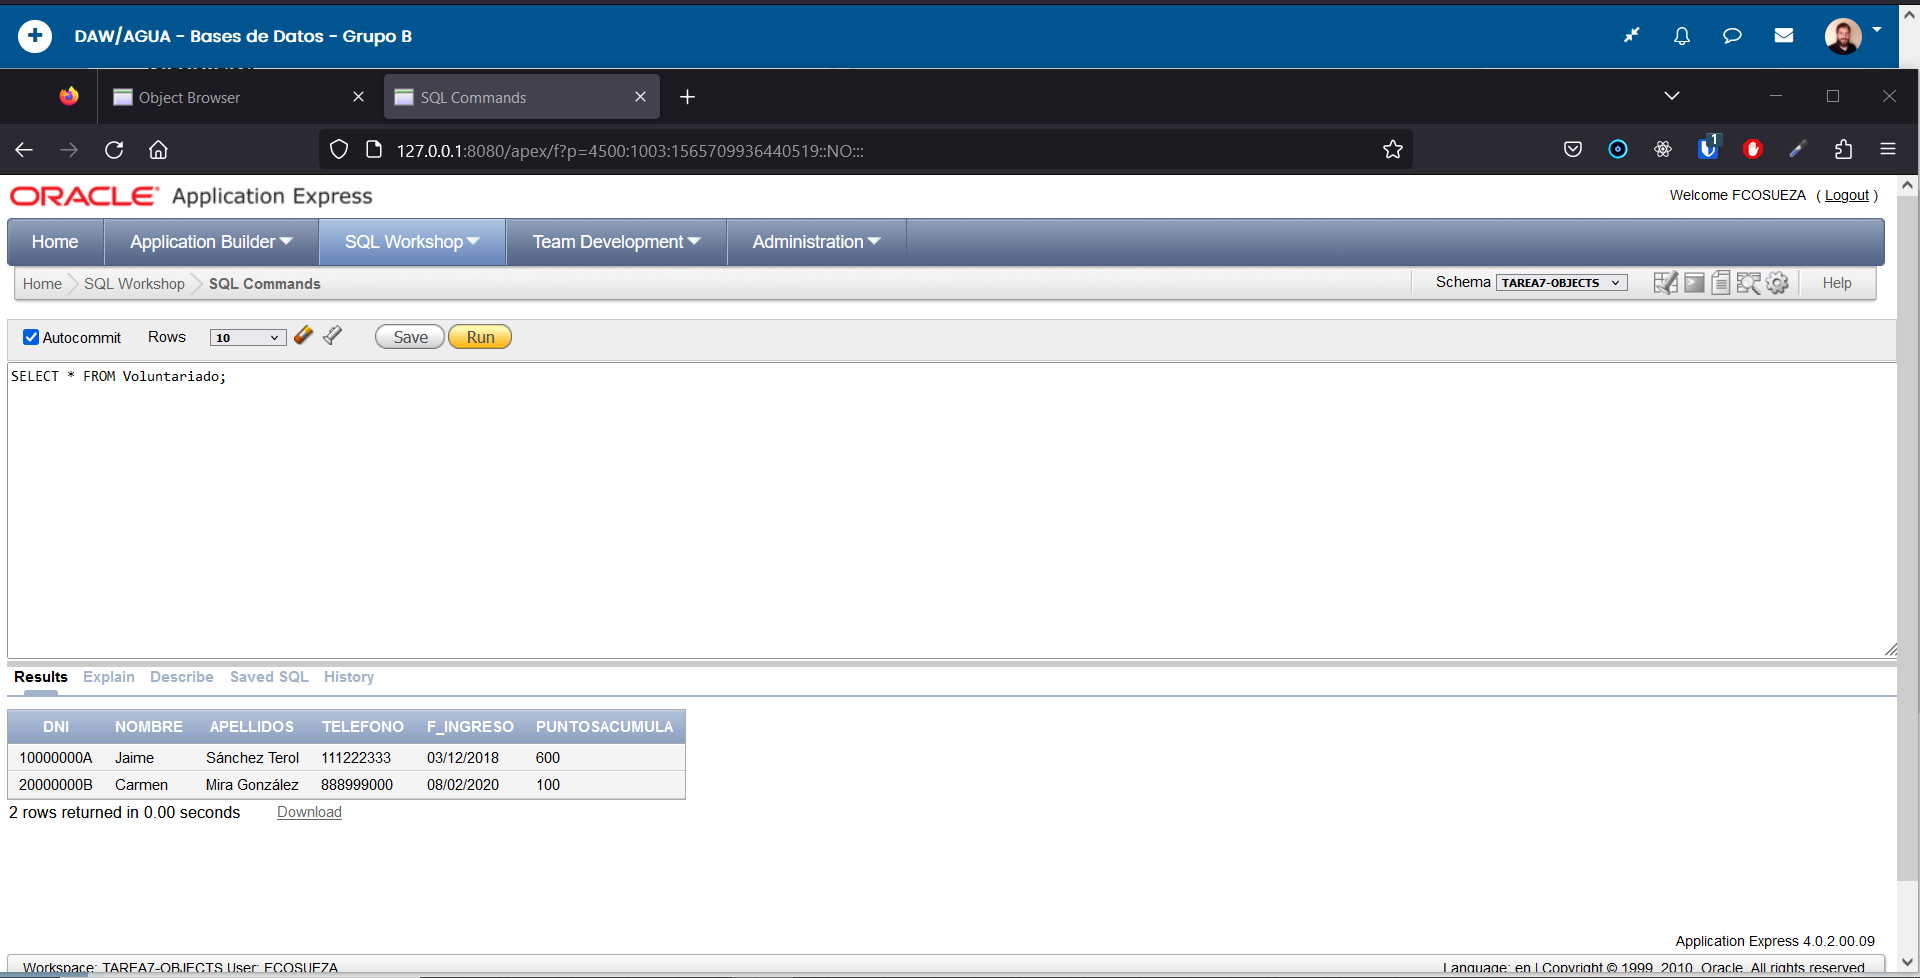
\includegraphics[scale=0.30]{voluntario-op-2.png}
        \caption{Tabla Voluntariado actualizad}
    \end{figure}

    El código empleado para este apartado ha sido el siguiente:

    \begin{figure}[H]
        \begin{tcolorbox}[sharp corners, colback=yellow!30, colframe=white!20]
            \tiny
            \begin{verbatim}
DECLARE
  voluntario_1 Voluntario;
  voluntario_2 Voluntario;
  puntos NUMBER;
BEGIN
  voluntario_1 := NEW Voluntario('10000000A', 'Jaime', 'Sánchez Terol', '111222333', TO_DATE('03/12/2018'), 200);
  voluntario_2 := NEW Voluntario('20000000B', 'Carmen', 'Mira González', '888999000', TO_DATE('08/02/2020'), 100);

  INSERT INTO Voluntariado VALUES(voluntario_1);
  INSERT INTO Voluntariado VALUES(voluntario_2);

  puntos := voluntario_1.calcularPuntosGanados(8);

  UPDATE Voluntariado SET Voluntariado.puntosAcumula = Voluntariado.puntosAcumula + puntos
  WHERE Voluntariado.DNI = '10000000A';
END;
            \end{verbatim}
        \end{tcolorbox}
    \end{figure}

    \item En este punto hemos trabajado con la tabla \textbf{Socios} creando varios y comprobando que el constructor que hemos creado funciona correctamente. Como vemos en la siguiente captura.

    \begin{figure}[H]
        \centering
        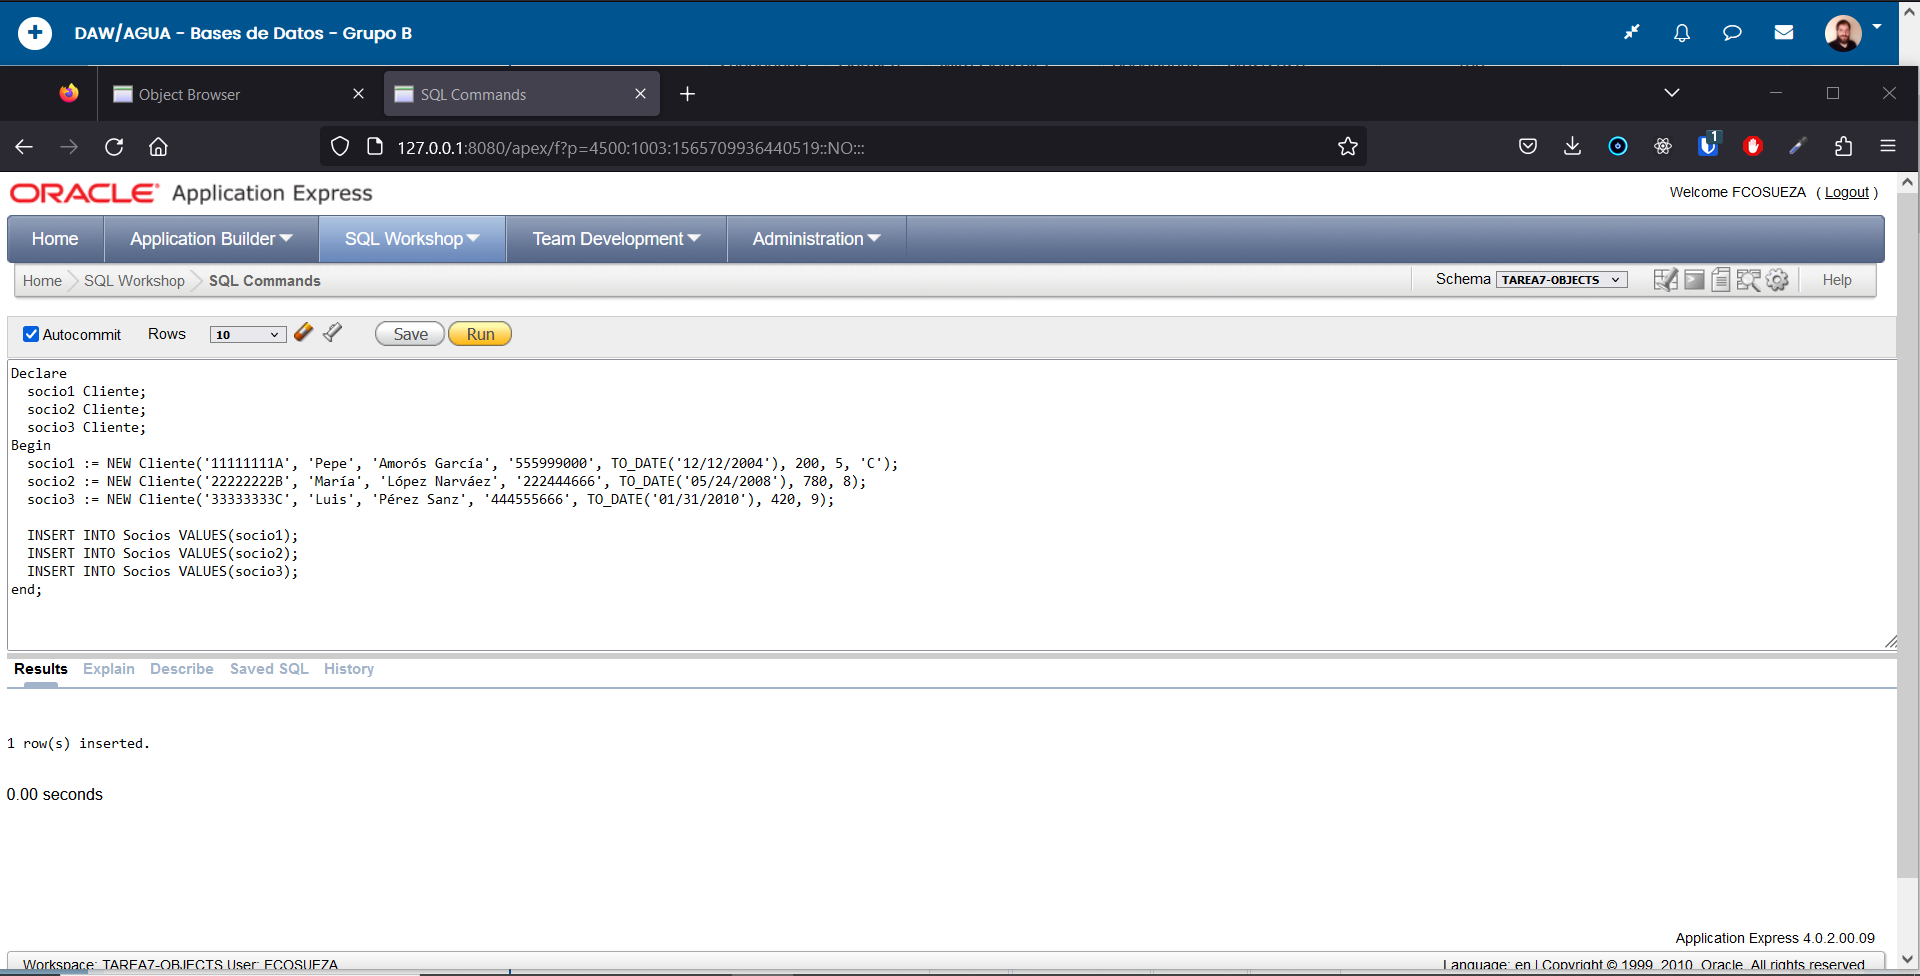
\includegraphics[scale=0.30]{socios-op-1.png}
        \caption{Creación e inserción de socios}
    \end{figure}

    Hemos comprobado que los datos se han creado correctamente, incluyendo el tipoAyuda generado automáticamente.

    \begin{figure}[H]
        \centering
        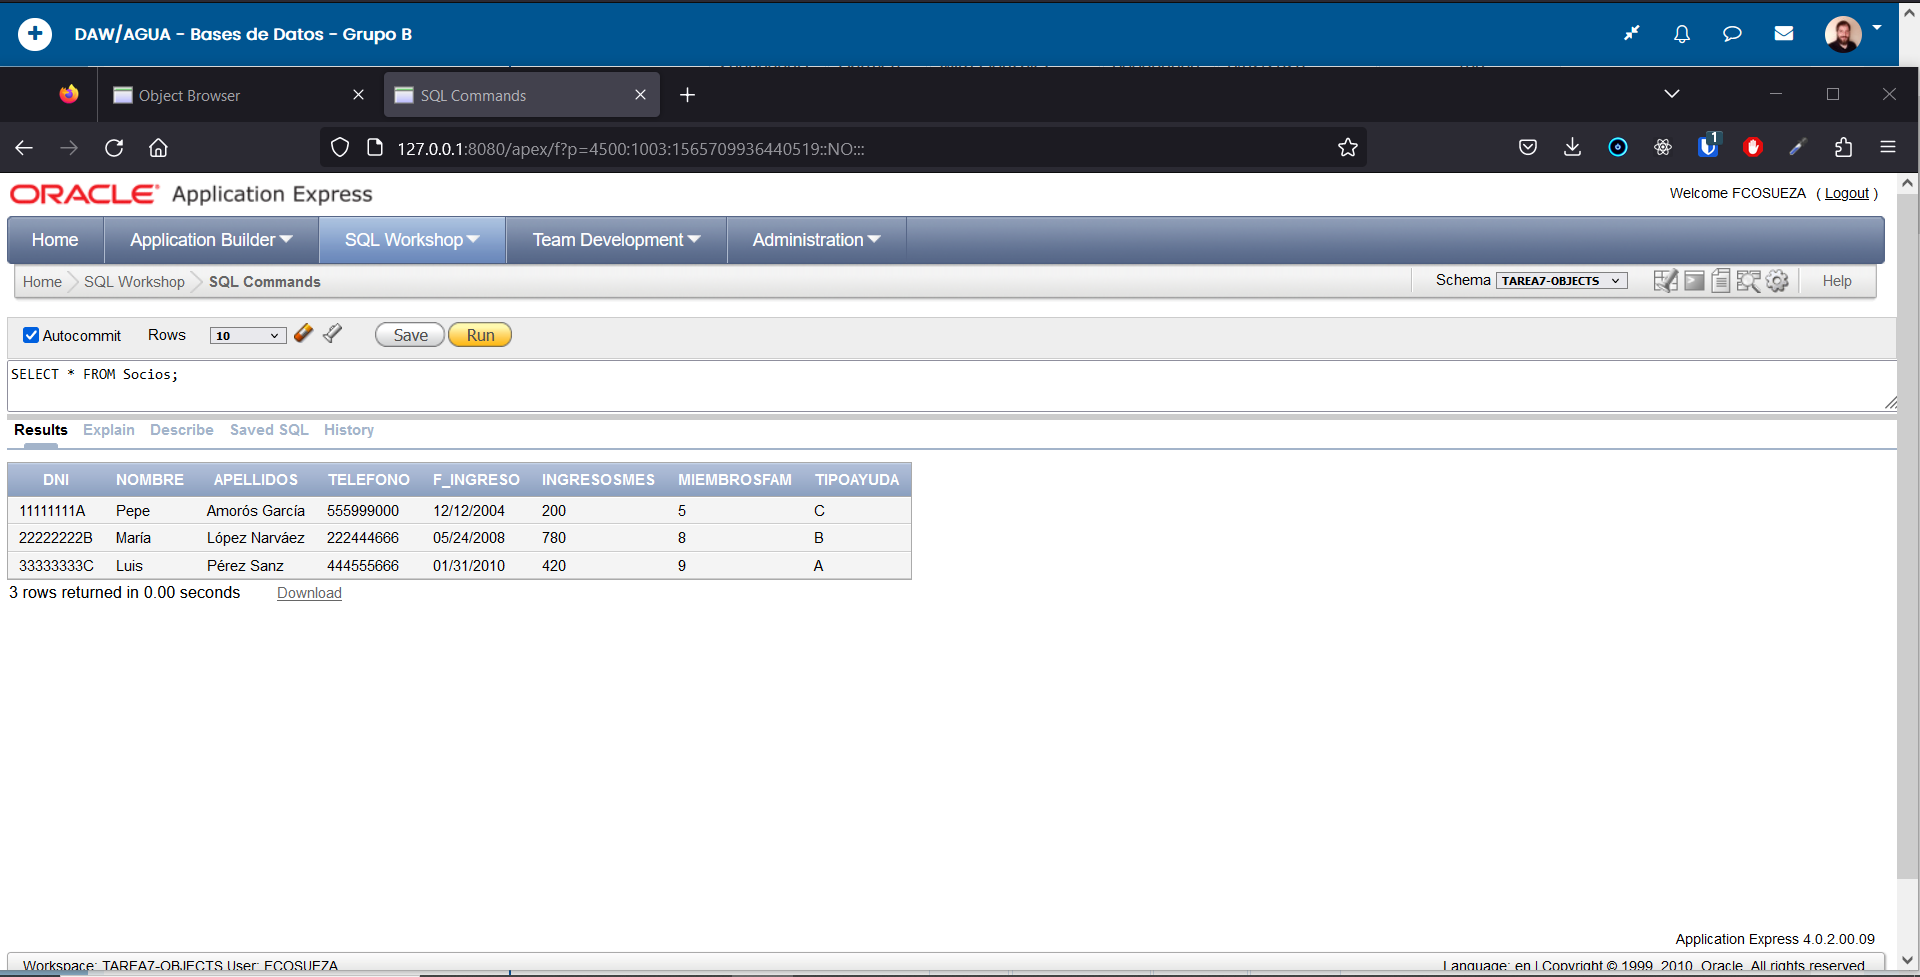
\includegraphics[scale=0.30]{socios-op-2.png}
        \caption{Tabla Socios actualizad}
    \end{figure}

    El código empleado a sido el siguiente:

    \begin{figure}[H]
        \begin{tcolorbox}[sharp corners, colback=yellow!30, colframe=white!20]
            \tiny
            \begin{verbatim}
Declare
  socio1 Cliente;
  socio2 Cliente;
  socio3 Cliente;
Begin
  socio1 := NEW Cliente('11111111A', 'Pepe', 'Amorós García', '555999000', TO_DATE('12/12/2004'), 200, 5, 'C');
  socio2 := NEW Cliente('22222222B', 'María', 'López Narváez', '222444666', TO_DATE('05/24/2008'), 780, 8);
  socio3 := NEW Cliente('33333333C', 'Luis', 'Pérez Sanz', '444555666', TO_DATE('01/31/2010'), 420, 9);

  INSERT INTO Socios VALUES(socio1);
  INSERT INTO Socios VALUES(socio2);
  INSERT INTO Socios VALUES(socio3);
end;
            \end{verbatim}
        \end{tcolorbox}
    \end{figure}
\end{enumerate}

\subsection{Actividad 5}
\subsubsection{Enunciado}
Realiza las siguientes operaciones sobre la tabla ENTREGADOS de forma independiente:
\begin{enumerate}[label=\alph*)]
    \item En primer lugar debes actualizar la fecha de la entrega con número 00004 con el nuevo valor 12/04/23. (Realiza una única sentencia SQL)
    \item Después y mediante un bloque PL/SQL recupera información de la tabla ENTREGADOS e imprime por pantalla la siguiente información sobre una entrega determinada cualquiera: (Aquí se muestra un ejemplo de lo que tendría que salir por pantalla si buscamos información sobre la entrega número 00002.) Puedes hacerlo con cualquier otro número de entrega.

    \begin{figure}[H]
        \centering
        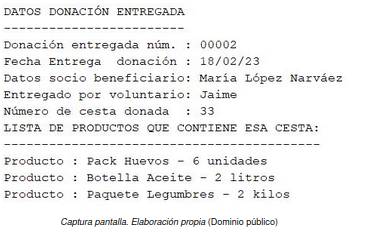
\includegraphics[scale=0.80]{ejemplo-salida-5.png}
    \end{figure}
\end{enumerate}

\subsubsection{Solución}
% Bibliography

%\newpage
%\bibliography{citas}
%\bibliographystyle{unsrt}

\end{document}